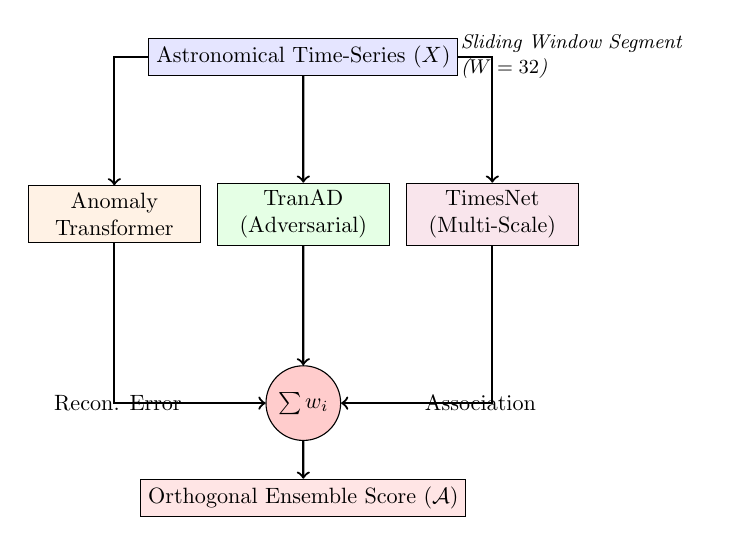
\begin{tikzpicture}[node distance=1.5cm, auto, scale=0.8, transform shape]
    % Nodes
    \node (input) [rectangle, draw, fill=blue!10, minimum width=3cm] {Astronomical Time-Series ($X$)};
    
    \node (trans) [rectangle, draw, fill=orange!10, below of=input, xshift=-3cm, yshift=-1cm, text width=2.5cm, align=center] {Anomaly\\Transformer};
    \node (tranad) [rectangle, draw, fill=green!10, below of=input, yshift=-1cm, text width=2.5cm, align=center] {TranAD\\(Adversarial)};
    \node (times) [rectangle, draw, fill=purple!10, below of=input, xshift=3cm, yshift=-1cm, text width=2.5cm, align=center] {TimesNet\\(Multi-Scale)};
    
    \node (gate) [circle, draw, fill=red!20, below of=tranad, yshift=-1.5cm] {$\sum w_i$};
    \node (output) [rectangle, draw, fill=red!10, below of=gate, minimum width=3cm] {Orthogonal Ensemble Score ($\mathcal{A}$)};
    
    % Connections
    \draw [->, thick] (input) -| (trans);
    \draw [->, thick] (input) -- (tranad);
    \draw [->, thick] (input) -| (times);
    
    \draw [->, thick] (trans) |- (gate) node[near end, left] {Recon. Error};
    \draw [->, thick] (tranad) -- (gate);
    \draw [->, thick] (times) |- (gate) node[near end, right] {Association};
    
    \draw [->, thick] (gate) -- (output);
    
    % Annotations
    \node [right of=input, xshift=3cm, text width=4cm, font=\small\itshape] {Sliding Window Segment ($W=32$)};
\end{tikzpicture}